\section{Motivation}\label{sec:motivation}

\subsection{Background}

The standard approach to FDE, using the AES \emph{block cipher}, introduces
significant overhead during filesystem operation. It is well known that
authenticated encryption using \emph{stream ciphers} like
ChaCha20~\cite{ChaCha20} is faster than using AES~\cite{StrongBox, AnotherPaper,
AnotherPaper}. However, when used naively in drive encryption, stream ciphers
are widely known to be vulnerable to ``overwrite attacks'' like pad reuse and
rollback~\cite{KatzLindell, StrongBox}. To enable FDE using stream ciphers,
several approaches have been explored:

\begin{itemize}
   \item Use a non-deterministic CTR mode with specially designed cipher and
   filesystem (Freestyle~\cite{Freestyle}).
   \item Use a length-preserving ``tweakable super-pseudorandom permutation''
   construction with nonce-accepting stream cipher (Adiantum~\cite{Adiantum}).
   \item Use a stream cipher in a binary additive (XOR) mode with metadata
   management to prevent overwrites (StrongBox~\cite{StrongBox}).
\end{itemize}

In this paper, we focus on the lattermost approach. StrongBox~\cite{StrongBox}
is a ChaCha20 stream cipher based FDE and metadata layer that exploits
Log-structured File Systems' (LFS) overwrite-averse behavior to achieve
high-performance encryption. StrongBox uses ChaCha20 in a secure binary additive
mode (XOR) to encrypt and decrypt data at rest. Threats like pad
reuse~\cite{KatzLindell} (\ie{two-time pad}) and rollback attacks---all caused
by overwrites---are mitigated through \emph{re-keying}, where groups of
contiguous storage blocks are decrypted with the old key and encrypted again
with a new key when an overwrite is detected. Unfortunately, re-keying is an
expensive operation. However, overwrite-averse LFS behavior ensures costly
re-keying operations are triggered as rarely as possible during I/O, preserving
or improving system performance~\cite{StrongBox}.

\begin{figure}[ht]
   \centering
   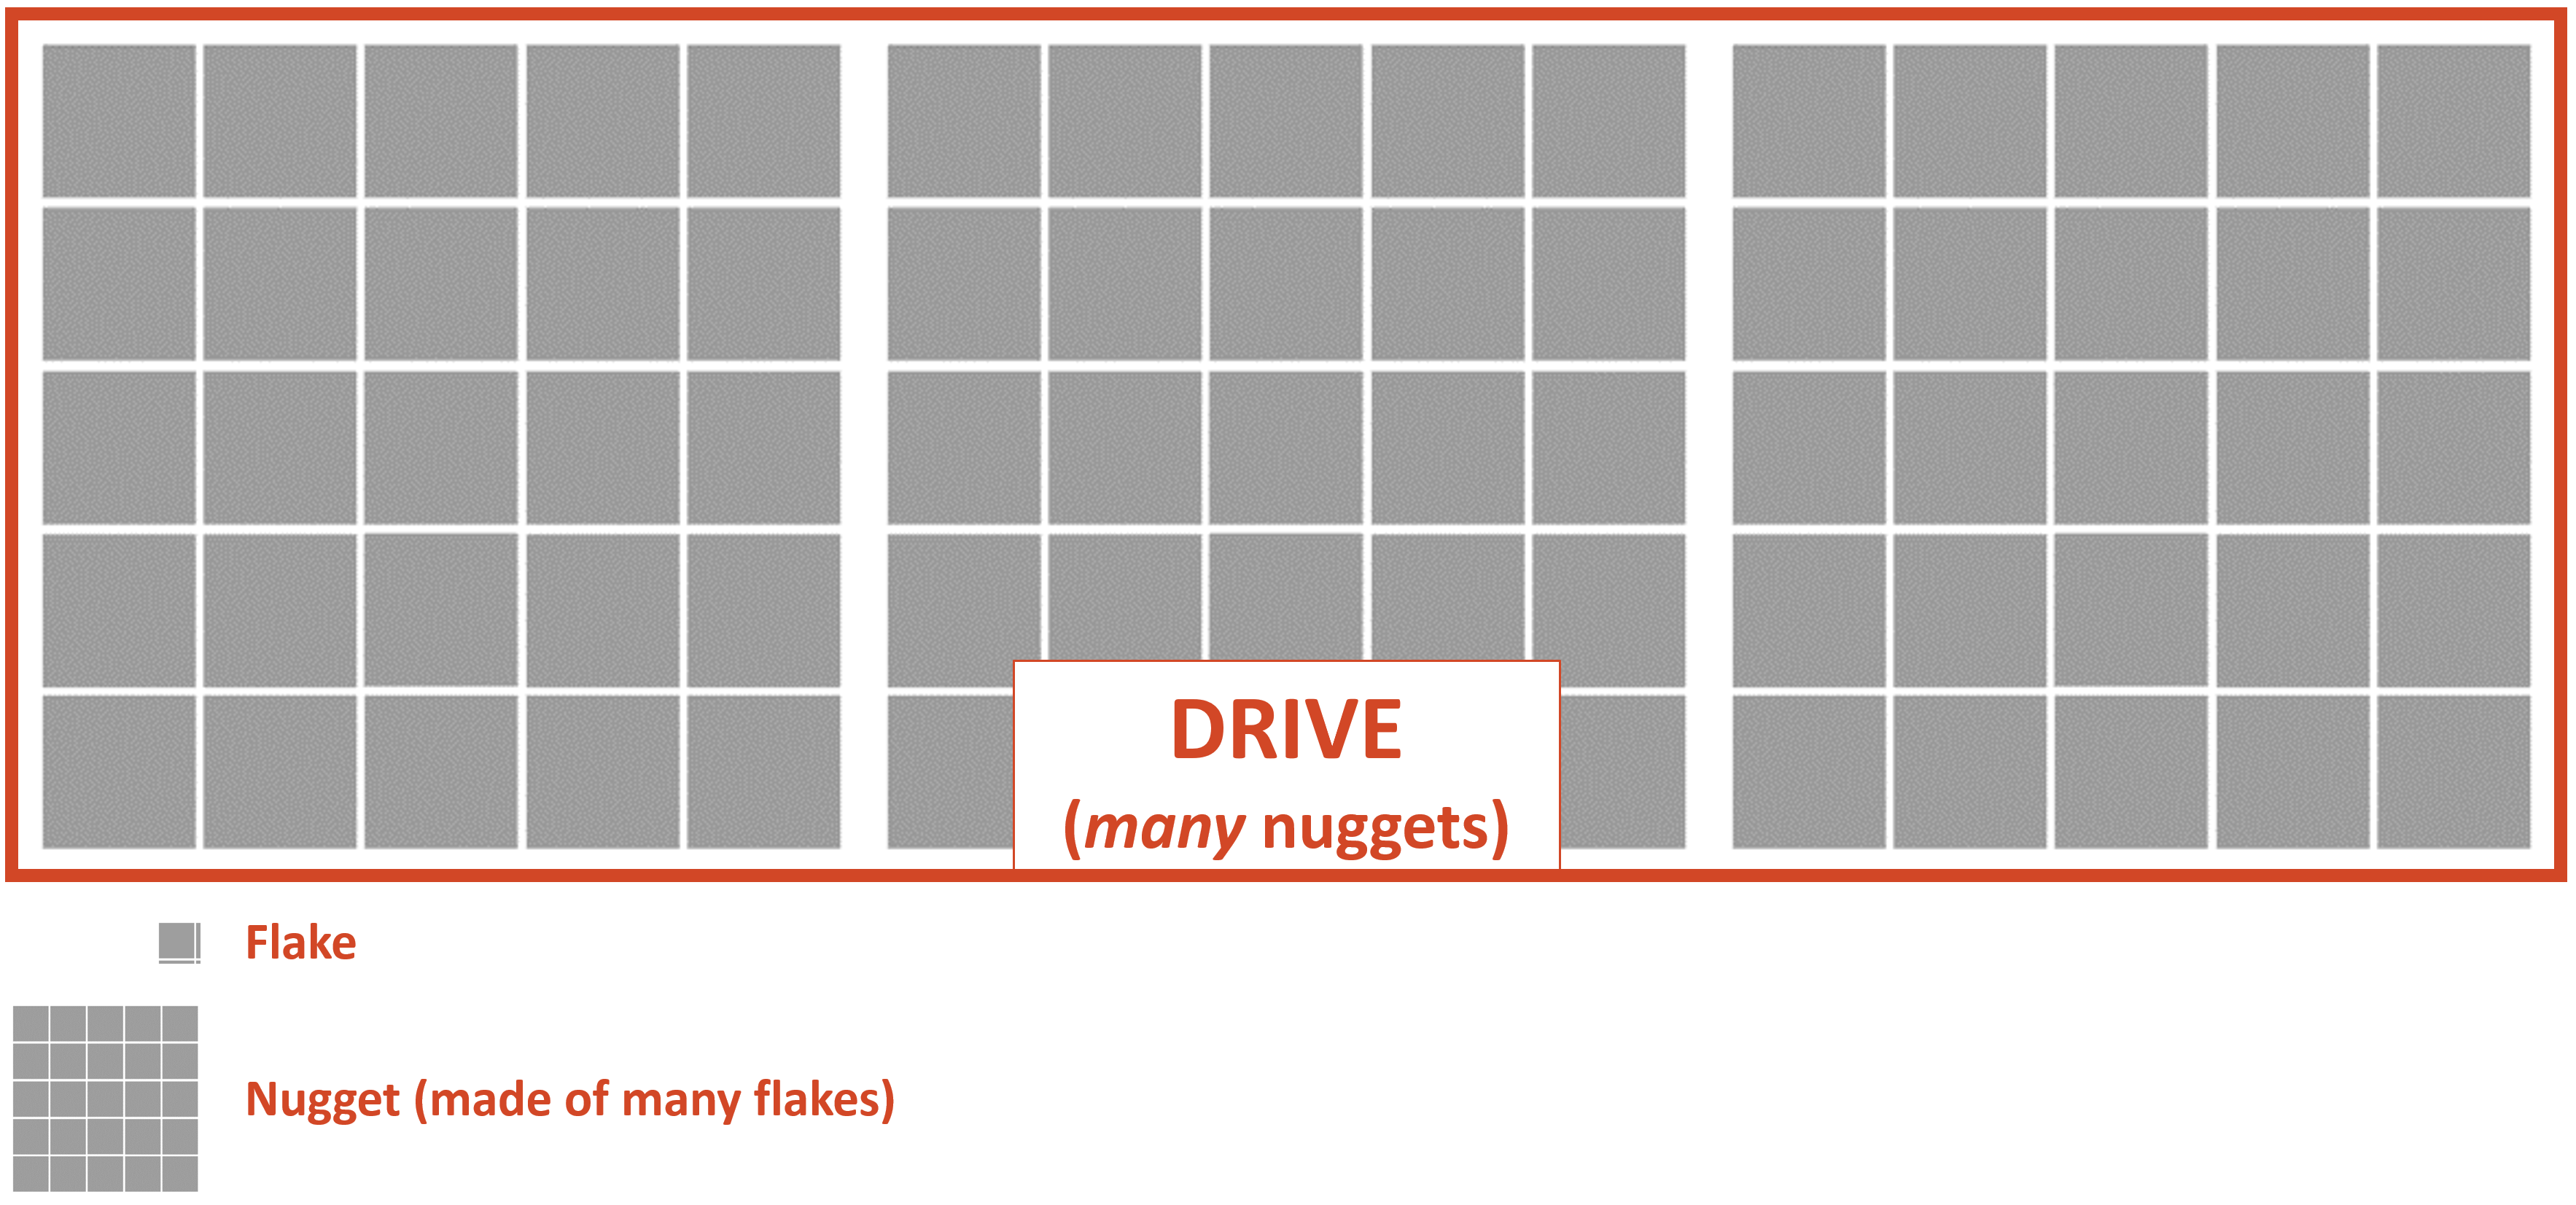
\includegraphics[width=\linewidth]{flknug.png}
   \caption{Anatomy of a StrongBox nugget.}\label{fig:flknug}
\end{figure}

StrongBox divides the underlying drive into a series same-size logical blocks
called \emph{nuggets}, illustrated in \figref{flknug}. A nugget consists of one
or more physical drive blocks/sectors, depending on its configured size. Each
nugget is subdivided into a constant number of units called \emph{flakes}.

This flake-nugget structure is used by StrongBox to 1) track, detect, and handle
overwrites and 2) limit the maximum length of any plaintexts provided to
ciphers, thus capping the per-cycle overhead incurred during expensive re-keying
operations when overwrites do occur.

\subsection{Key Insights}

\subsubsection{A Single Point In A Space Of Possible Cipher Configurations}

What if we used StrongBox with \textit{ciphers} other than ChaCha20? Redesigning
StrongBox with a generic cipher API allows for ciphers other than ChaCha20 to be
used, yielding a space of cipher configuration points with various performance,
battery life, security, drive space, and other tradeoffs. It follows then that
the original StrongBox construction using ChaCha20 exists as one point in this
space of cipher configurations.

\begin{figure}[ht]
   \centering
   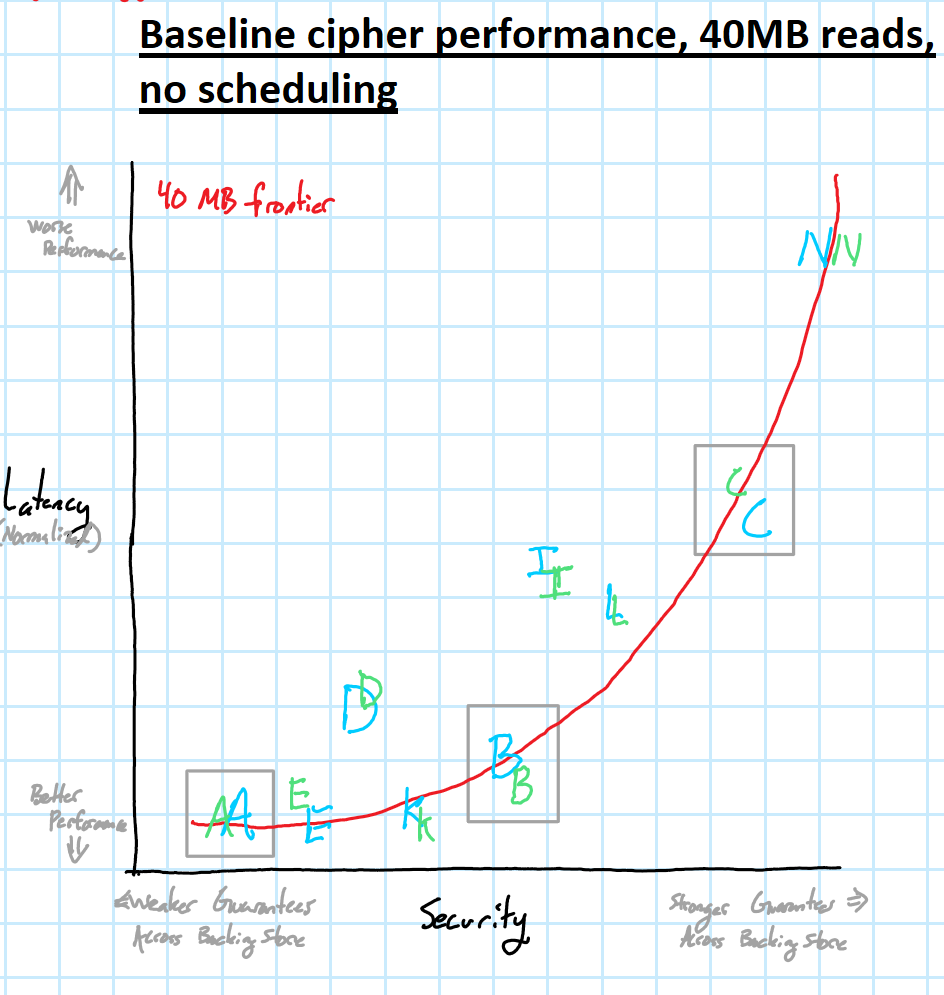
\includegraphics[width=\linewidth]{drawn/1.png}
   \caption{\TODO{Caption goes here}\TODO{No curve in this version!}}\label{fig:40mb-read}
\end{figure}

For instance, \figref{40mb-read} shows the security versus I/O latency tradeoff
between different stream ciphers (including ChaCha20) when completing a 40MB
read of encrypted storage. The experiment was performed on a Linux RAM disk on
an ARM big.LITTLE Exynos Octa processor, which is similar to the processors used
in the Samsung Galaxy line of phones and other devices. Of the ciphers we
tested, those with more desirable but performance inhibitive security guarantees
(see: \secref{design}) resulted in higher latency for I/O operations while
ciphers with relatively weaker less desirable security guarantees resulted in
lower latency.

\subsubsection{Nugget Encryption/Decryption And Re-Keying Is Entirely Independent}

With SwitchBox, nuggets are considered as distinct logical blocks, each with
their own metadata and unique cryptographic key used to encrypt and decrypt
their contents independent of other nuggets using the cipher chosen at system
initialization. This layout of distinct logical blocks naturally lends itself to
encrypting different portions of the underlying drive with different ciphers
instead; we can select any cipher to encrypt or decrypt any nugget at any point,
rather than just a single cipher applied globally across the backing store. This
allows the system to support mixed cipher configurations that can be encrypted,
decrypted, switched individually.

\subsubsection{Navigate The Configuration Space With ``Cipher Switching''}

Given a space of possible cipher configurations and a drive layout of
independent nuggets that lends itself to mixed cipher use, it is clear our
system does not have to sit at a static configuration point. Hence, we require a
mechanism to navigate the cipher configuration space, trading off concerns such
that the system is always at the most optimal configuration given the runtime
environment. By abstracting the re-keying process out into a \emph{re-ciphering}
or \emph{cipher switching} process, whereby the key and the cipher used to
encrypt/decrypt the nugget can both be switched at runtime, we can trade off
between different ciphers and their characteristics dynamically. Comparatively,
prior work can only accomplish a static tradeoff at compile time or at
system initialization. \\
\\
Leveraging these insights, we present SwitchBox. \TODO{A few short explanatory
sentences that lead to: Our goal is to dynamically trade desirable security
properties for performance or energy.}

\subsection{Motivating Example: Filesystem Reacts to OS ``Power Saver'' Mode}

\begin{figure}[ht]
   \centering
   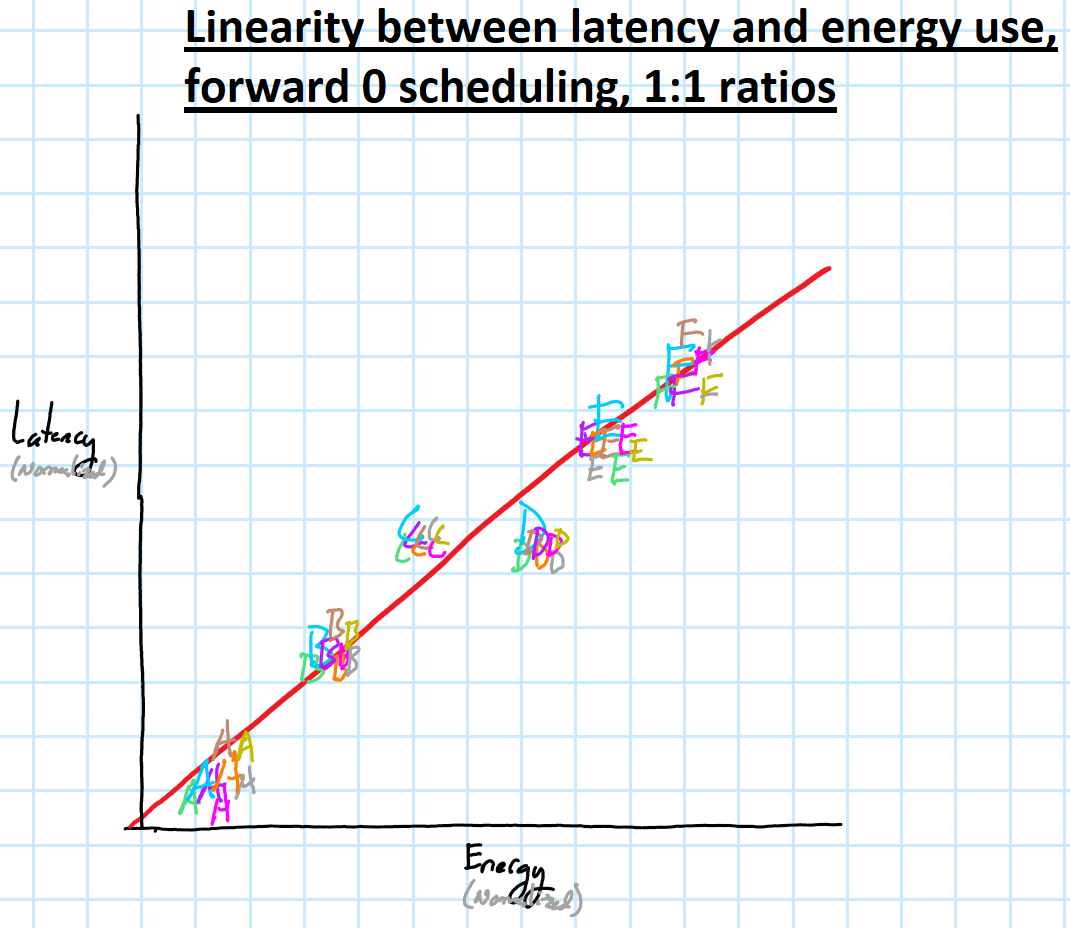
\includegraphics[width=\linewidth]{drawn/5.png}
   \caption{\TODO{Caption goes here}}\label{fig:energy-latency-linearity}
\end{figure}

Suppose we are continually streaming a high-resolution video stored on our
mobile device to several WiFi connected devices, such as televisions or
projectors. We stored the video and other data on our device drive as securely
as possible, so we chose to initialize the system at a configuration point
offering very strong security.

For the ciphers examined in this paper, \figref{energy-latency-linearity} shows
a correlation between stronger security guarantees and greater total energy use,
meaning our device is using a lot more energy to facilitate FDE at this
configuration point. Though this correlation applies to the ciphers we examined,
note that this correlation is certainly not true for all possible ciphers.

Further suppose that, after a while of streaming, our device determines its
remaining battery life is too low and enters a ``power saver'' mode with a
curtailed energy budget. With a traditional filesystem or encrypted container, we
are stuck with our high-energy configuration chosen at system initialization.

However, with the ability to operate at points along the pareto frontier (see
\figref{40mb-read}), even at points between the discrete configurations
available to prior work, a context-aware system can switch to a configuration
that trades the security of the portions of storage that are being used to
stream the video so that we stay within our curtailed energy budget.

When we return to a non-curtailed energy budget, the system can return to its
more secure configuration dynamically, allowing the cipher strength of the
backing store to eventually recover without having to recreate the entire
underlying filesystem or encrypted container.

\subsection{Challenges}

\textbf{Comparing ciphers with disparate security guarantees.} To ensure that
these tradeoffs are made optimally, it is desirable to score the security
properties of various ciphers. This is challenging since different ciphers have
a wide range of energy/latency vs security properties, including ciphers that
are and are not length-preserving. Hence, cipher configurations won't form a
continuous tradeoff space in any scheme and so represent discrete points, yet
the most optimal configuration state may lie between these points.

To address this, we propose a method for quantitative cipher comparison in the
FDE context, and then present some empirical results showing the wide range of
security and energy tradeoffs that become available with various
state-of-the-art ciphers as a result.\\
\\
\textbf{Maintaining I/O performance with a mixed-cipher drive layout.} With
prior work, cipher configurations are typically fixed at the time the system is
booted or the filesystem or container is created~\cite{CiteAllTheFilesystems}; if
requirements change online, at best the entire system requires a reboot which is
not optimal. At worst, before the reboot, the filesystem or encrypted container
has to be deleted and recreated. This is rarely desirable. Hence, SwitchBox
requires a generic \emph{cipher API}, IPC, and a software mechanism that can
re-cipher or \emph{switch} the cipher used to encrypt and decrypt individual
nuggets while maintaining low overhead and acceptable performance. This
mechanism should allow for a mixed-cipher drive layout and provides the ``how''
to switch nuggets' ciphers.

To provide the ``when'' or ``where'', we implement and demonstrate a series of
novel cipher switching \textit{strategies} that, along with the ``pluggable''
cipher API and cipher switching mechanism, enable optimal navigation of the
tradeoff space of configurations. For instance, these strategies allow SwitchBox
to settle on points between the static cipher configurations in
\figref{40mb-read}.

\TODO{Might be able to piece this out into two challenges: common interface for
stream ciphers and cipher switching strategies; that last one might be able to
split into two on its own. Perhaps this challenge subsection should mirror the
layout of the design section?}
